%%%%%%%%%%%%%%%%%%%%%%%%%%%%%%%%%%%%%%%%%
% Beamer Presentation
% LaTeX Template
% Version 1.0 (10/11/12)
%
% This template has been downloaded from:
% http://www.LaTeXTemplates.com
%
% License:
% CC BY-NC-SA 3.0 (http://creativecommons.org/licenses/by-nc-sa/3.0/)
%
%%%%%%%%%%%%%%%%%%%%%%%%%%%%%%%%%%%%%%%%%

%----------------------------------------------------------------------------------------
%	PACKAGES AND THEMES
%----------------------------------------------------------------------------------------

\documentclass{beamer}

\mode<presentation> {

% The Beamer class comes with a number of default slide themes
% which change the colors and layouts of slides. Below this is a list
% of all the themes, uncomment each in turn to see what they look like.

%\usetheme{default}
%\usetheme{AnnArbor}
%\usetheme{Antibes}
%\usetheme{Bergen}
%\usetheme{Berkeley}
%\usetheme{Berlin}
%\usetheme{Boadilla}
%\usetheme{CambridgeUS}
%\usetheme{Copenhagen}
%\usetheme{Darmstadt}
%\usetheme{Dresden}
%\usetheme{Frankfurt}
%\usetheme{Goettingen}
%\usetheme{Hannover}
%\usetheme{Ilmenau}
%\usetheme{JuanLesPins}
%\usetheme{Luebeck}
%\usetheme{Madrid}
%\usetheme{Malmoe}
%\usetheme{Marburg}
%\usetheme{Montpellier}
%\usetheme{PaloAlto}
%\usetheme{Pittsburgh}
%\usetheme{Rochester}
%\usetheme{Singapore}
\usetheme{Szeged}
%\usetheme{Warsaw}

% As well as themes, the Beamer class has a number of color themes
% for any slide theme. Uncomment each of these in turn to see how it
% changes the colors of your current slide theme.

%\usecolortheme{albatross}
\usecolortheme{beaver}
%\usecolortheme{beetle}
%\usecolortheme{crane}
%\usecolortheme{dolphin}
%\usecolortheme{dove}
%\usecolortheme{fly}
%\usecolortheme{lily}
%\usecolortheme{orchid}
%\usecolortheme{rose}
%\usecolortheme{seagull}
%\usecolortheme{seahorse}
%\usecolortheme{whale}
%\usecolortheme{wolverine}

%\setbeamertemplate{footline} % To remove the footer line in all slides uncomment this line
%\setbeamertemplate{footline}[page number] % To replace the footer line in all slides with a simple slide count uncomment this line

%\setbeamertemplate{navigation symbols}{} % To remove the navigation symbols from the bottom of all slides uncomment this line
}

\usepackage{graphicx} % Allows including images
\usepackage{booktabs} % Allows the use of \toprule, \midrule and \bottomrule in tables
\usepackage{hyperref}
\usepackage{xcolor}

%----------------------------------------------------------------------------------------
%	TITLE PAGE
%----------------------------------------------------------------------------------------

\title[CEBAF]{The Continuous Electron Beam Accelerator Facility at Jefferson Lab} % The short title appears at the bottom of every slide, the full title is only on the title page

\author{Matt Solt} % Your name
\institute[Stanford] % Your institution as it will appear on the bottom of every slide, may be shorthand to save space
{
SLAC National Accelerator Laboratory \\ % Your institution for the title page
\medskip
\textit{mrsolt@slac.stanford.edu} % Your email address
}
\date{\today} % Date, can be changed to a custom date

\begin{document}

\begin{frame}
\titlepage % Print the title page as the first slide
\end{frame}

%----------------------------------------------------------------------------------------
%	PRESENTATION SLIDES
%----------------------------------------------------------------------------------------

%------------------------------------------------
%\section{First Section} % Sections can be created in order to organize your presentation into discrete blocks, all sections and subsections are automatically printed in the table of contents as an overview of the talk
%------------------------------------------------

%\subsection{Subsection Example} % A subsection can be created just before a set of slides with a common theme to further break down your presentation into chunks

\begin{frame}
\frametitle{Introduction}
\begin{itemize}
\item The \textbf{Continuous Electron Beam Accelerator Facility} (CEBAF) is a recirculating linac at Jefferson Laboratory in Newport News, VA dedicated to studying the interface of nuclear and particle physics
\item One such type of experiment is the \textbf{Heavy Photon Search} (HPS) which searches for hidden sector vector bosons (i.e. fundamental forces)
\item HPS requires a high intensity continuous beam with low tails and low emittance in y
\item CEBAF provides such a facility - an overview and key design considerations will be presented
\end{itemize}

\end{frame}

%------------------------------------------------

\begin{frame}
\frametitle{Evidence for Extra Forces in Nature}
\begin{itemize}
\item Very strong evidence for \textbf{extra invisible matter} in the universe (dark matter) seen through galactic rotation curves, gravitational lensing, and CMB
\item WIMPs are most popular candidate but have not detected
\item Possibility for lighter dark matter - \textbf{requires a new mediator} (Lee-Weinberg Bound at 2 GeV)
\begin{figure}
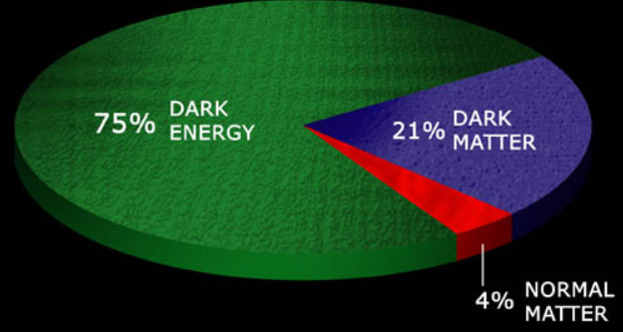
\includegraphics[width=0.60\linewidth]{figs/darkmatter.png}
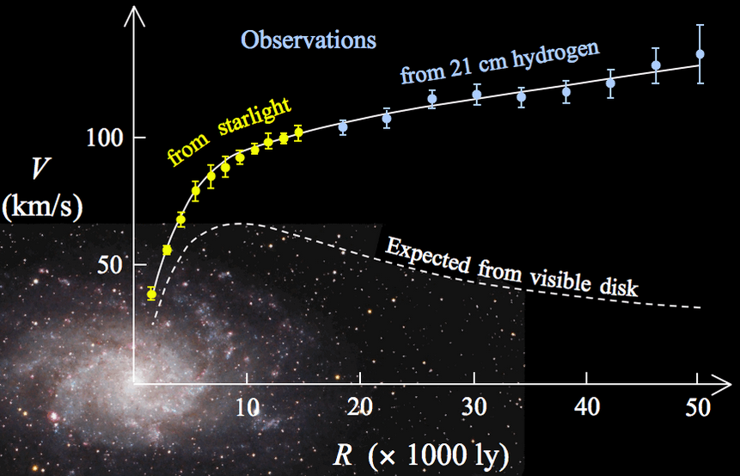
\includegraphics[width=0.50\linewidth]{figs/galaxy.png}
\end{figure}
\end{itemize}

\end{frame}

%------------------------------------------------

\begin{frame}
\frametitle{Signatures for Extra Forces}
\begin{itemize}
\item Some models predict an \textbf{extra massive U(1) symmetry} in nature where the force carrier (A') that can decay to lepton pairs (HPS left) invisible particles (LDMX right)
\begin{figure}
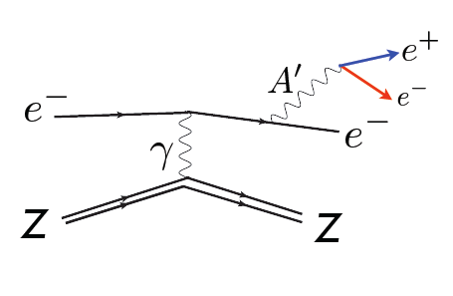
\includegraphics[width=0.30\linewidth]{figs/visible_decay.png}
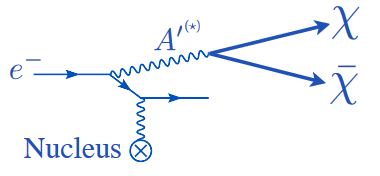
\includegraphics[width=0.30\linewidth]{figs/invisible_decay.png}
\end{figure}
\begin{figure}
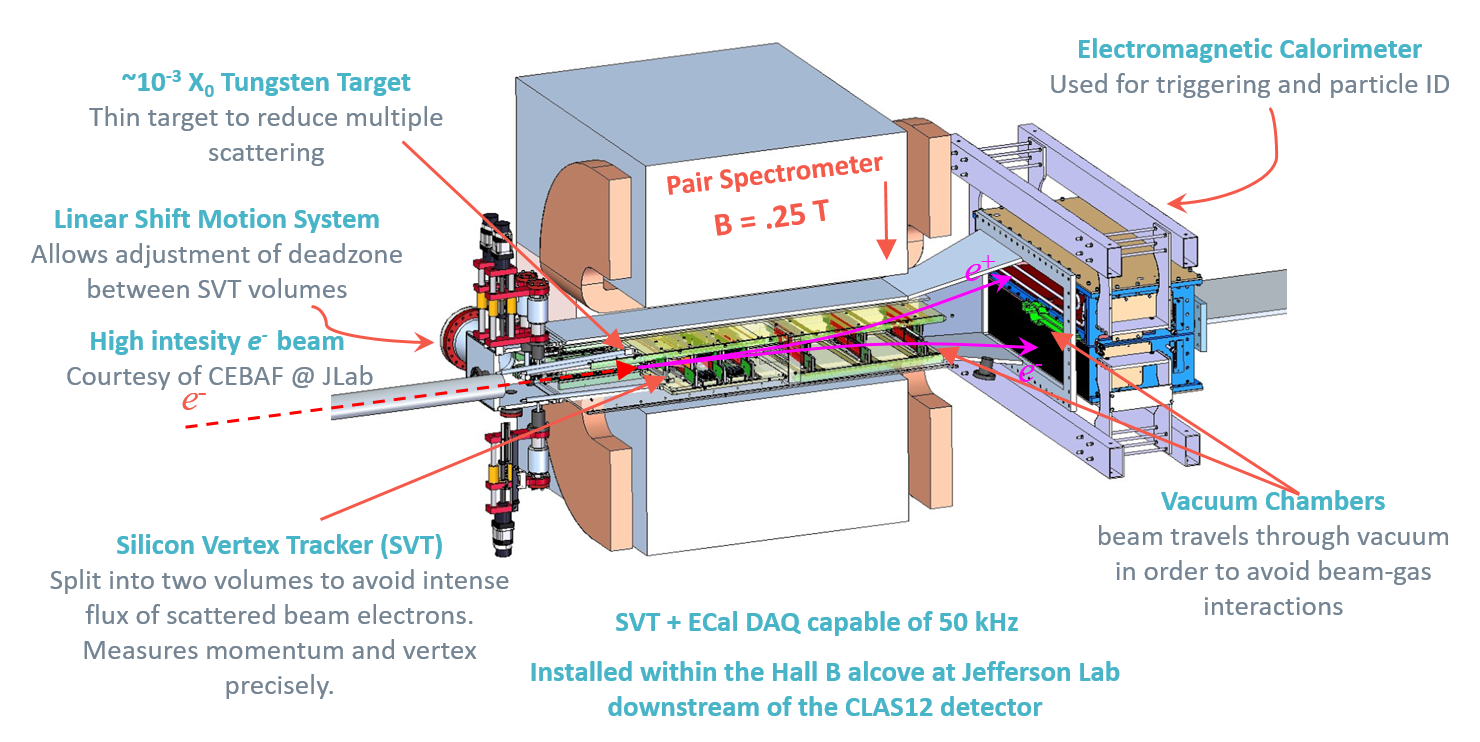
\includegraphics[width=0.60\linewidth]{figs/hps.png}
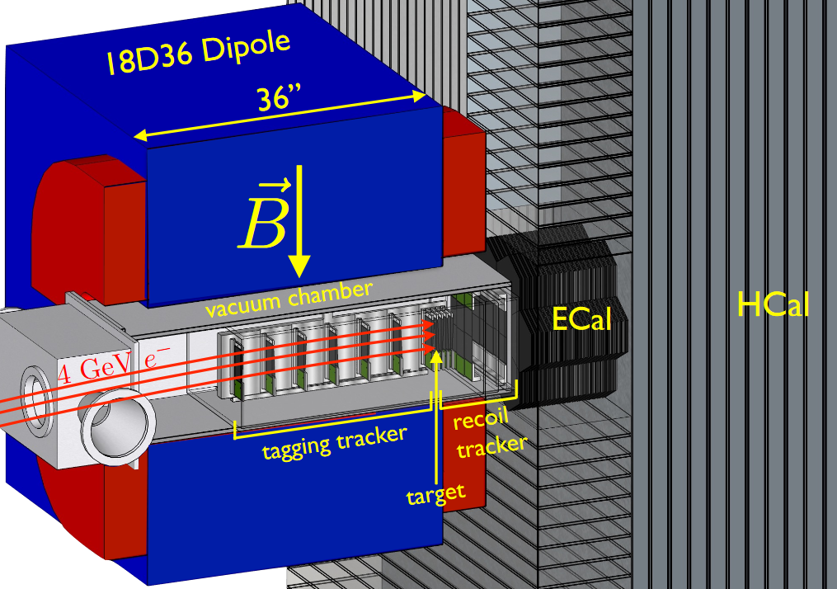
\includegraphics[width=0.45\linewidth]{figs/LDMX.png}
\end{figure}
\end{itemize}

\end{frame}

%------------------------------------------------

\begin{frame}
\frametitle{Heavy Photon Parameter Space}
\begin{figure}
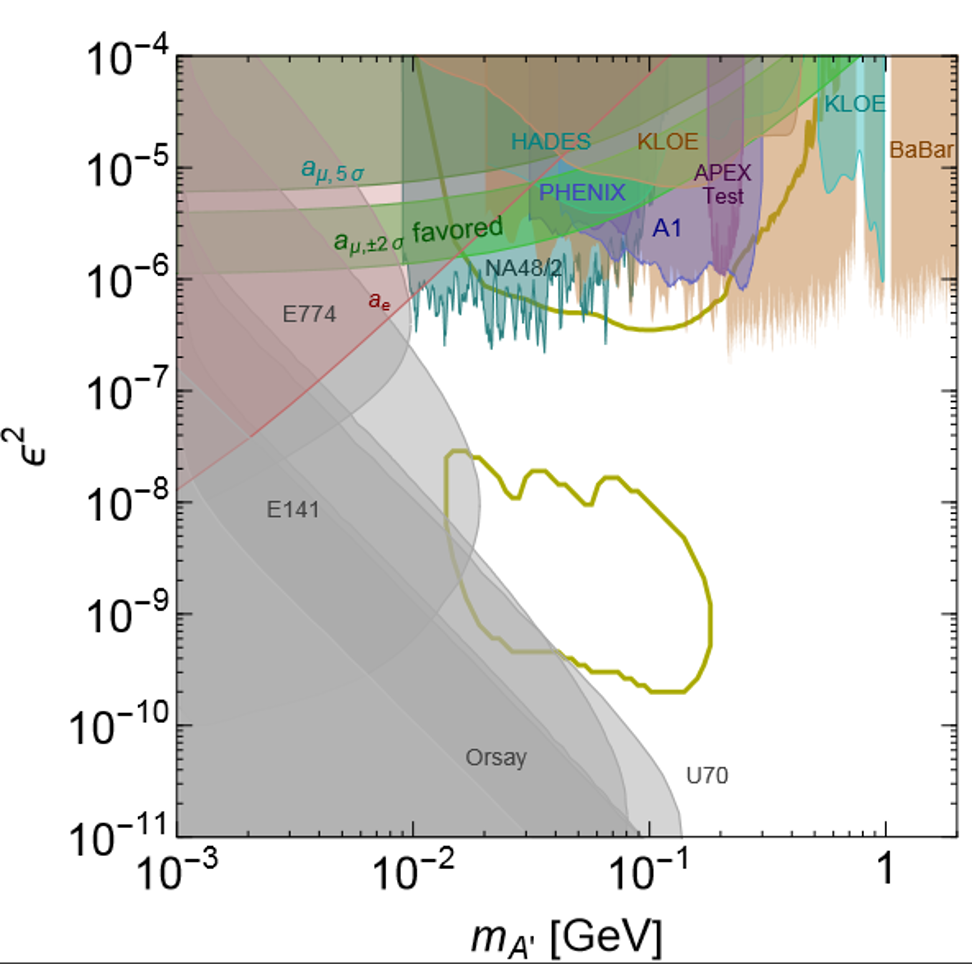
\includegraphics[width=0.65\linewidth]{figs/reach1.png}
\end{figure}

\end{frame}

%------------------------------------------------

\begin{frame}
\frametitle{Heavy Photon Parameter Space}
\begin{figure}
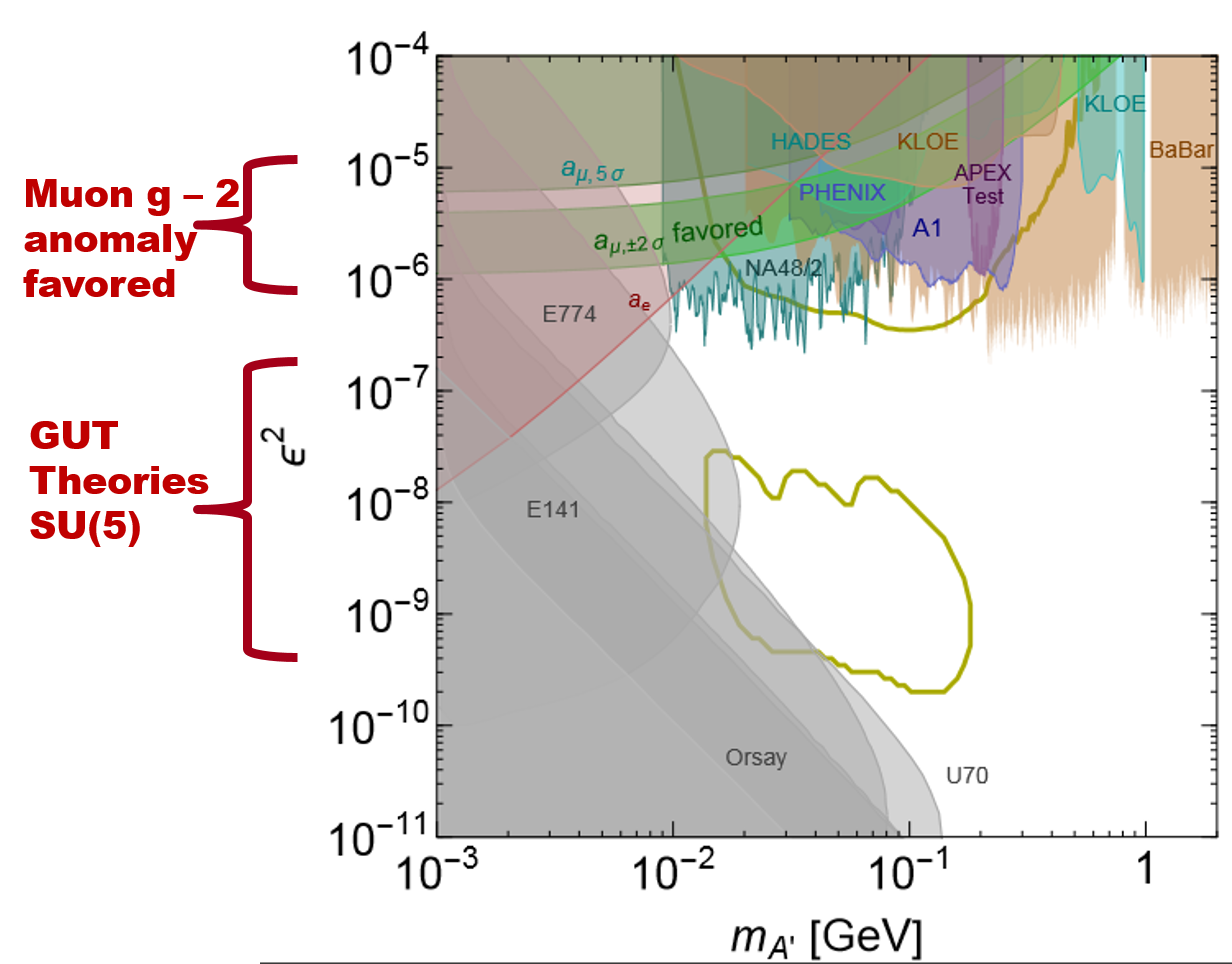
\includegraphics[width=0.80\linewidth]{figs/reach2.png}
\end{figure}

\end{frame}

%------------------------------------------------

\begin{frame}
\frametitle{Heavy Photon Parameter Space}
\begin{figure}
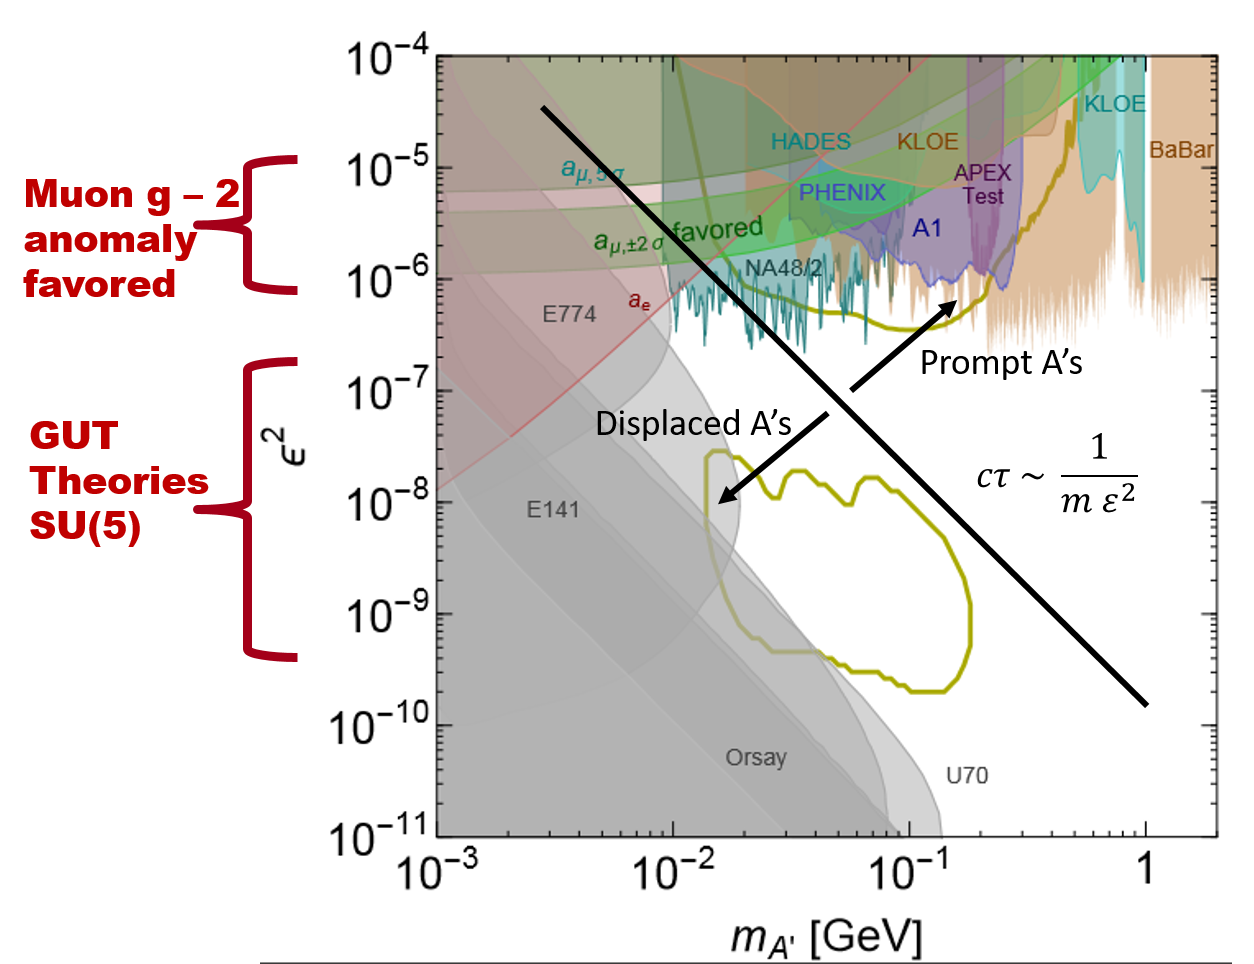
\includegraphics[width=0.80\linewidth]{figs/reach3.png}
\end{figure}

\end{frame}

%------------------------------------------------

\begin{frame}
\frametitle{Heavy Photon Parameter Space}
\begin{figure}
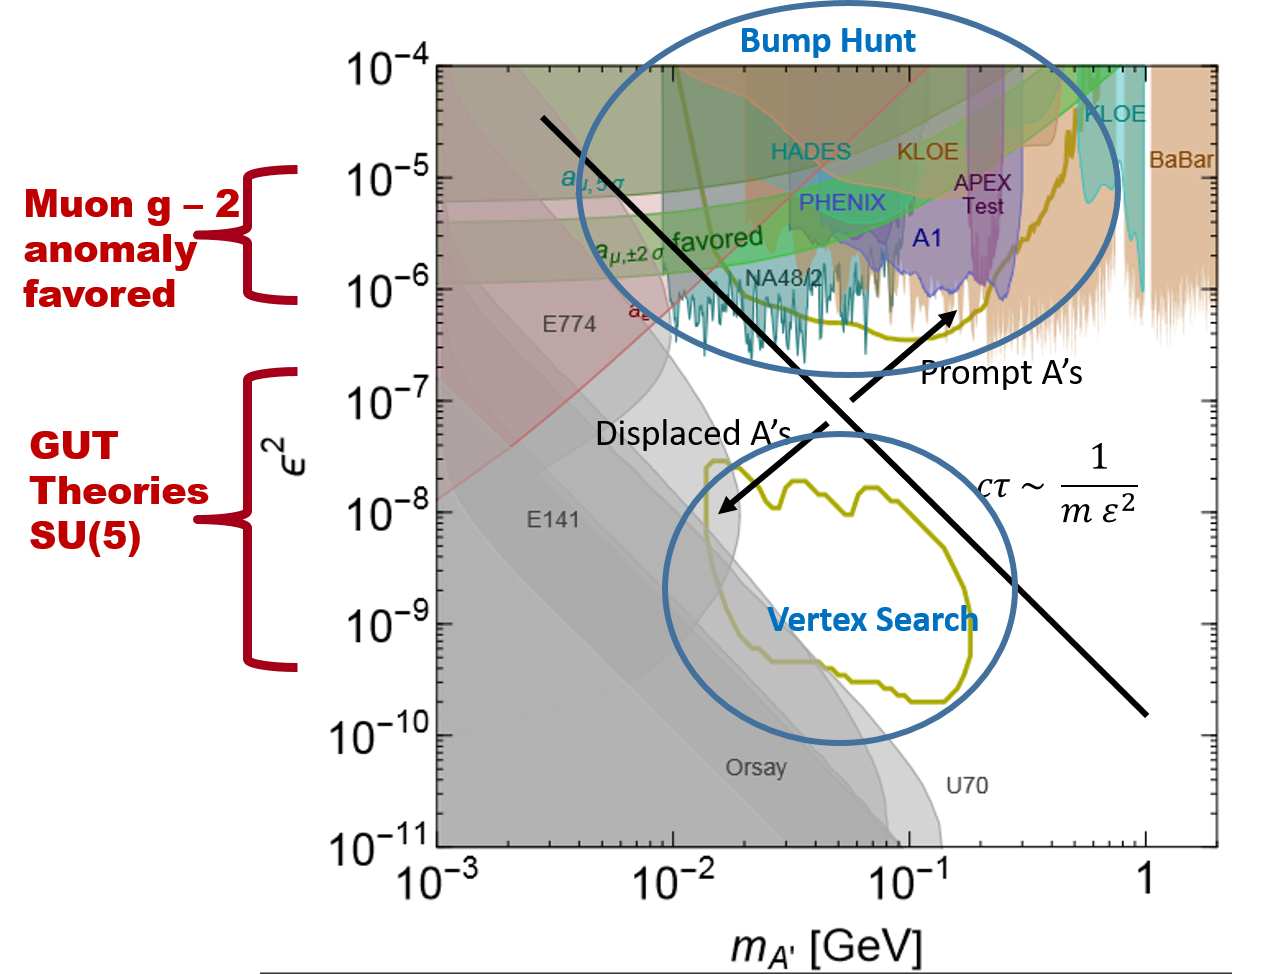
\includegraphics[width=0.80\linewidth]{figs/reach4.png}
\end{figure}

\end{frame}

%------------------------------------------------

\begin{frame}
\frametitle{HPS Beam Requirement}
\begin{itemize}
\item HPS requires intermediate beam energies, flat beam with low tails and halo, and excellent position stability
\end{itemize}
\begin{figure}
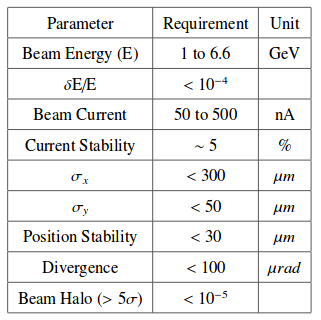
\includegraphics[width=0.50\linewidth]{figs/beam_parameters.png}
\end{figure}

\end{frame}

%------------------------------------------------

\begin{frame}
\frametitle{CEBAF}
\begin{itemize}
\item CEBAF is a five-pass recirculating srf linac located at Jefferson Lab in Newport News, VA. \textbf{Capable of simulatneously delivering intense electron beams of different energies and currents} to 4 experimental halls (2.2 GeV/pass).
\end{itemize}
\begin{figure}
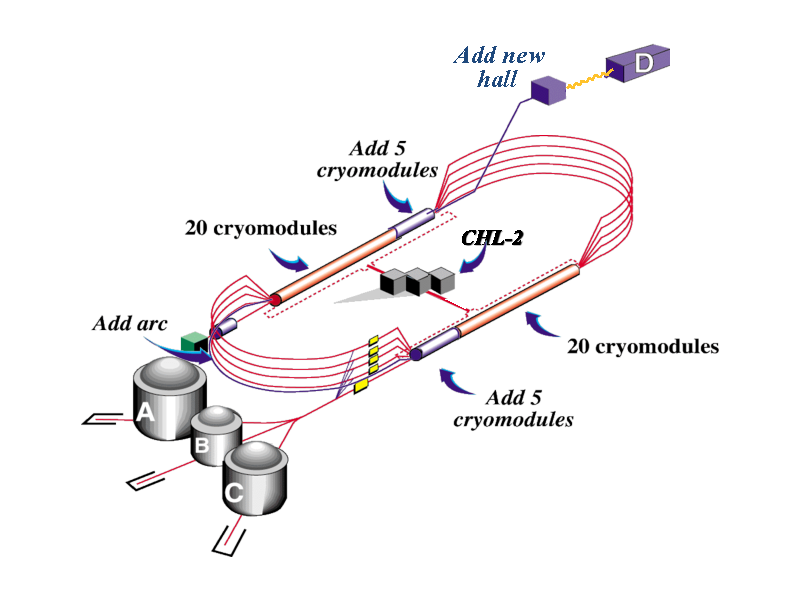
\includegraphics[width=0.65\linewidth]{figs/CEBAF.png}
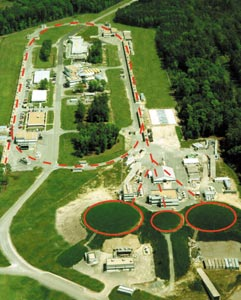
\includegraphics[width=0.35\linewidth]{figs/CEBAF2.jpg}
\end{figure}

\end{frame}

%------------------------------------------------

\begin{frame}
\frametitle{History of CEBAF}
\begin{itemize}
\item High enery physics explores quark-quark interactions ($>\approx$100 GeV). Nuclear physics explores nucleon-nucleon interactions ($<\approx$1 GeV)
\item In 1980's, there was a consensus to explore nuclear physics at the transition between these (intermediate energy physics). Also good for high intensity particle physics experiments
\begin{figure}
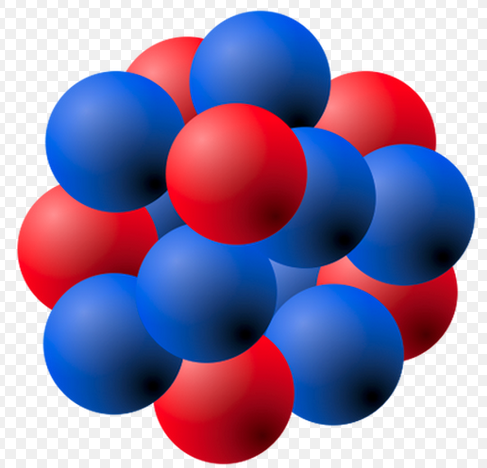
\includegraphics[width=0.35\linewidth]{figs/nucleons.png}

\includegraphics[width=0.35\linewidth]{figs/arrow.png}
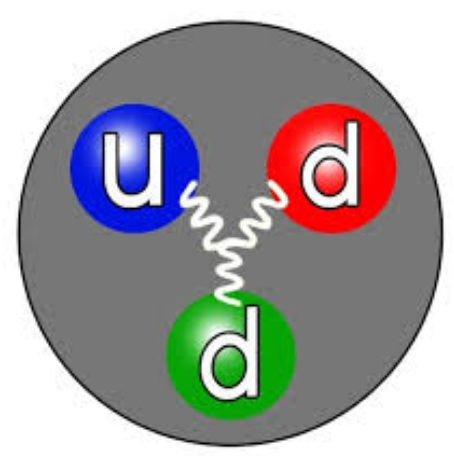
\includegraphics[width=0.35\linewidth]{figs/quarks.png}
\end{figure}
\end{itemize}

\end{frame}

%------------------------------------------------

\begin{frame}
\frametitle{CEBAF Recirculation and SRF Cavities}
\begin{itemize}
\item \textbf{Largest scale for srf technology and recirculating linac at the time}
\item Srf technology drastically reduced operating costs, but still needed to adopt beam recirculation (linac section needs to be $\frac{1}{n}$ the length of a full-energy linac where $n$ is the number of passes)
\end{itemize}
\begin{figure}
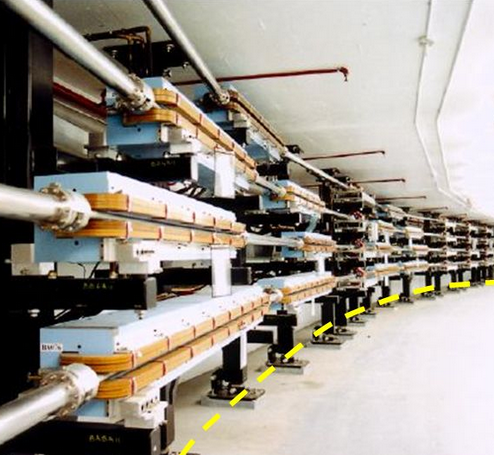
\includegraphics[width=0.50\linewidth]{figs/arc.png}
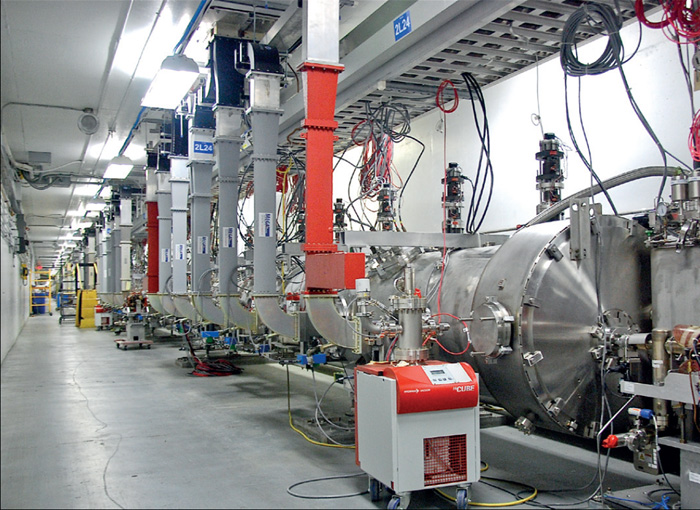
\includegraphics[width=0.60\linewidth]{figs/srf.jpg}
\end{figure}

\end{frame}

%------------------------------------------------

\begin{frame}
\frametitle{CEBAF SRF Cavities}
\begin{itemize}
\item Construction began in 1987. Each five-cell cavity is 0.5 m long (total of 160 cavities) and total active linac length is 4.5 km
\item \textbf{$f_{rf}$ operates at 1497 MHz} and a acceleration gradient of 5 MV/m
\item Each linac contains 20 cryomodules of srf cavities (now 25 for 12 GeV upgrade)
\end{itemize}
\begin{figure}
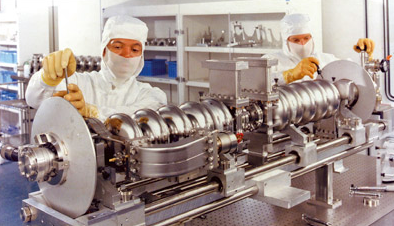
\includegraphics[width=0.50\linewidth]{figs/srf_cavities.png}
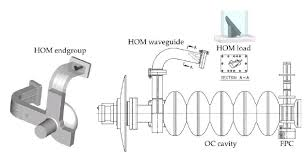
\includegraphics[width=0.50\linewidth]{figs/srf_schematic.jpeg}
\end{figure}

\end{frame}

%------------------------------------------------

\begin{frame}
\frametitle{CEBAF Beam Pulse}
\begin{itemize}
\item Each transports system must accommodate the unique momentum of beam after each pass
\item In accelerating sections, \textbf{bunches of different energy occupy the same space}. Each pulse is directed into a different hall
%\item linac-to-linac system must be isochronous and achromatic on all passes ($M_{56}<0.1 $m)
\item Bend sections are generous enough to allow for a 12 GeV
\begin{figure}
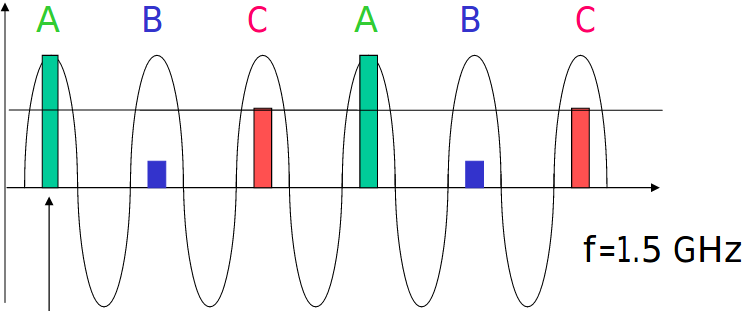
\includegraphics[width=0.65\linewidth]{figs/beam_pulses.png}
\end{figure}
\end{itemize}
\end{frame}


%------------------------------------------------

\begin{frame}
\frametitle{12 GeV CEBAF Upgrade}
\begin{itemize}
\item Ten new higher-voltage cryomodules, i.e., superconducting radio-frequency (SRF) accelerating elements (five per Linac).
\item Ten new RF stations to power the 10 new cryomodules.
\item Approximately double the refrigeration capacity.
\item Modifications to the magnets in the recirculation arcs and their power supplies to keep the higher energy beam confined to the existing beam path.
\item Modifications to the extraction system to support the higher energy beams.
\item A tenth arc-beamline to provide an extra pass through the North Linac. This additional acceleration pass will bring the beam up to the 12 GeV required to accommodate the experimental program in the \textbf{new hall (Hall D)}.
\item A new beamline connecting Hall D to the baseline accelerator.
\item Room for a 24 GeV upgrade in the future
\end{itemize}

\end{frame}

%------------------------------------------------

\begin{frame}
\frametitle{CEBAF RF Separators}
\begin{itemize}
\item RF separators are installed at the end of each pass to deflect beams (about 0.1 mrad)
\item After some drifting, septa magnets direct beam to another pass or to the experimental halls
\item Another RF separator directs beam to Hall A, B, and C
\end{itemize}
\begin{figure}
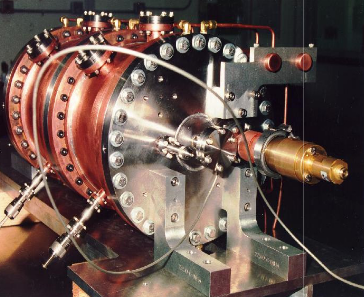
\includegraphics[width=0.35\linewidth]{figs/rf_kicker.png}
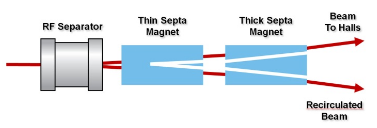
\includegraphics[width=0.70\linewidth]{figs/rf_separator2.png}
\end{figure}

\end{frame}

%------------------------------------------------

\begin{frame}
\frametitle{CEBAF RF Separators}
\begin{itemize}
\item RF separators operate at 500 MHz ($\frac{1}{3} f_{rf}$) and can direct either beam 2 (left) or 3 (right) different directions
\item Hall D requires a new RF separator at the last pass for 12 GeV and operates at 750 MHz ($\frac{1}{2} f_{rf}$)
\end{itemize}
\begin{figure}
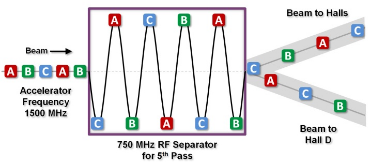
\includegraphics[width=0.35\linewidth]{figs/500MHz_rf_separator.png}
\end{figure}
\begin{figure}
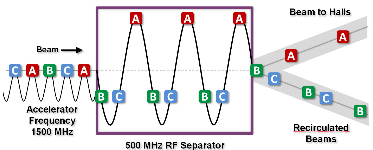
\includegraphics[width=0.50\linewidth]{figs/beam_separator3.png}
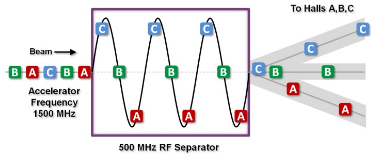
\includegraphics[width=0.50\linewidth]{figs/beam_separator4.png}
\end{figure}

\end{frame}

%------------------------------------------------

\begin{frame}
\frametitle{CEBAF Polarized Electron Source}
\begin{itemize}
\item Polarizated electron beams are extremely useful for spin-dependent physics but was not a part of the original CEBAF design
\item Polarization $P_e$ is defined $P_e=\frac{N_+-N_-}{N}$ where $N_+$ and $N_-$ are spin up and down electrons, respectively, and $N$ is the total number of electrons
\item CEBAF obtains about 80\% polarization and begins at the source
\item CEBAF uses photoemission from GaAs as a polarized electron source (first done at SLAC for parity violation)
\end{itemize}
%\begin{figure}
%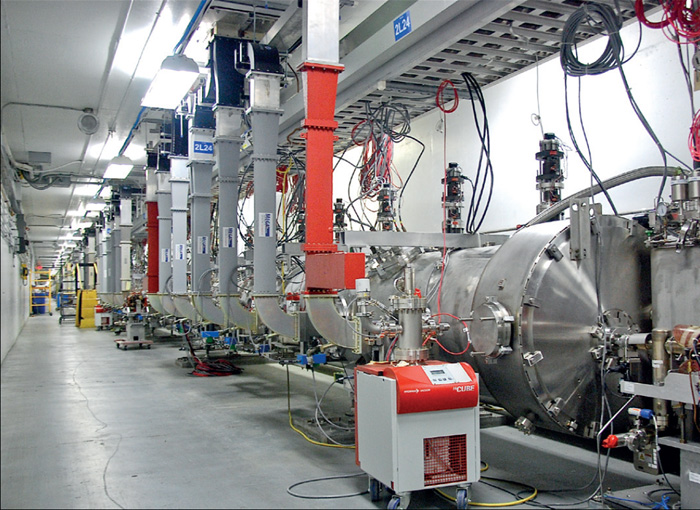
\includegraphics[width=0.35\linewidth]{figs/srf.png}
%\end{figure}

\end{frame}

%------------------------------------------------

\begin{frame}
\frametitle{CEBAF Polarized Electron Source}
\begin{itemize}
\item User a laser to selectively populate a the conduction band with electrons of a particular spin state
\item Some of these electrons diffuse to the surface and some leave the material (but more of a particular spin state)
\item One can reduce the work function by p-doping the GaAs, and one monolayer of Cs and oxidant reduces the work function below the conduction band
\end{itemize}
\begin{figure}
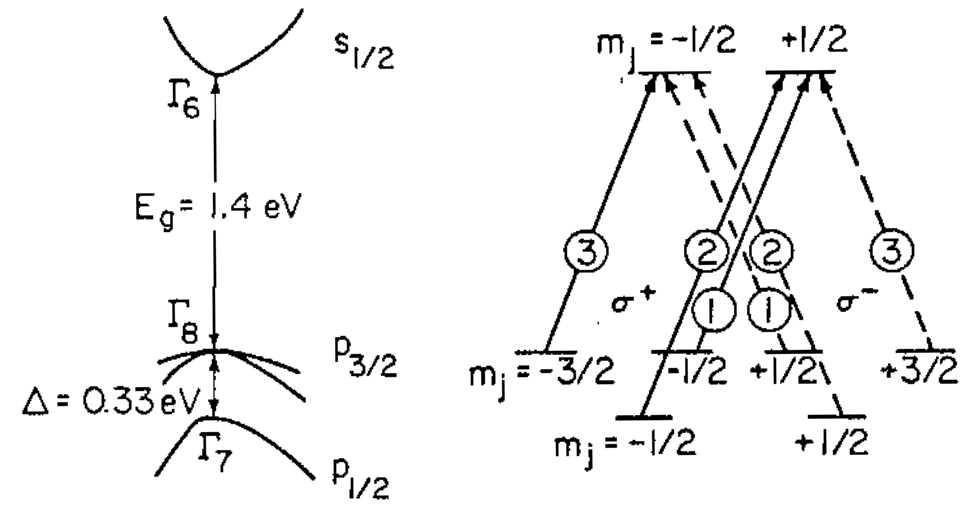
\includegraphics[width=0.50\linewidth]{figs/band_structure.png}
\end{figure}

\end{frame}

%------------------------------------------------

%\begin{frame}
%\frametitle{CEBAF Polarized Electron Source}
%\begin{itemize}
%\item band
%\end{itemize}
%\begin{figure}
%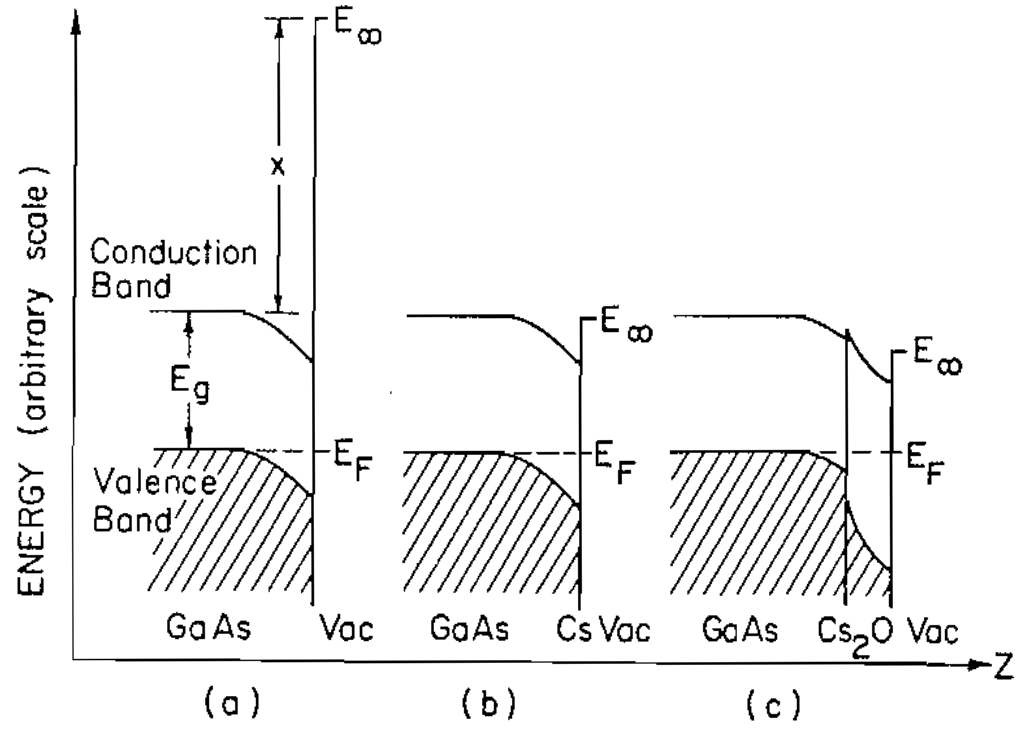
\includegraphics[width=0.35\linewidth]{figs/ptype_band_structure.png}
%\end{figure}

%\end{frame}

%------------------------------------------------

\begin{frame}
\frametitle{Beam Breakup Instability}
\begin{itemize}
\item Concerns about multiple pass beam breakup. A beam passing off-axis through a cavity excites deflecting higher-order modes
\item \textbf{Beam breakup severely limits current} in superconducting linacs due to inherently high Q's of transverse deflecting modes of the rf cavities
\item This can happen in both longitudinal and transverse directions
%\item Degradation of beam quality must be minimized, phase-space dilution could occur due to synchrotron radiation excitation during recirculation
%\item Arcs must be achromatic, isochronous, and have beam-path length that is an integer multiple of $\lambda_{rf}$
%\item Synchrotron radiation-induced phase-space degradation must be minimized
\begin{figure}
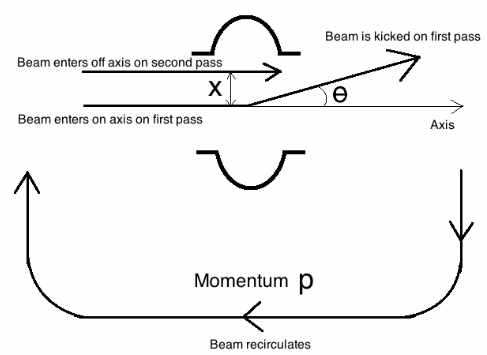
\includegraphics[width=0.60\linewidth]{figs/recirculation.png}
\end{figure}
\end{itemize}
\end{frame}

%------------------------------------------------

%\begin{frame}
%\frametitle{Beam Breakup}
%\begin{itemize}
%\item Hi
%\end{itemize}
%\begin{equation}
%\sigma_E^2=1.182 \times 10^{-33} \mathrm{GeV}^2 \mathrm{m}^2 \frac{\gamma^7}{\rho^2}
%\end{equation}
%\begin{equation}
%\Delta \epsilon = 1.32 \pi \times 10^{-27} \mathrm{m}^2 \mathrm{rad} \frac{\gamma^5}{\rho^2} \left\langle H \right\rangle
%\end{equation}
%\begin{equation}
%\left\langle H \right\rangle = \frac{1}{L} \int_{arcs} ds \ \frac{1}{\beta} \left(\eta^2+ \left(\beta \eta'-\frac{1}{2} \beta' \eta \right)^2 %\right)
%\end{equation}

%\end{frame}

%------------------------------------------------

\begin{frame}
\frametitle{Beam Breakup Theory}
\begin{itemize}
\item CEBAF srf runs using $\mathrm{TM}_{010}$ mode (non-zero $E$ field on cylinder axis), however higher order modes (HOMs) of $\mathrm{TM}_{mnp}$ and $\mathrm{TE}_{mnp}$, or parasitic modes, can be \textbf{induced externally from beam particles}
\item Off axis beam particles produce a transverse wake at a given HOM $W_{\lambda}$ which is a function of cavity impedance $R/Q$, HOM wavenumber $k_{\lambda}$, HOM frequency $\omega_{\lambda}$, and loaded quality factor $Q_{\lambda}$
\end{itemize}
\begin{equation}
W_{\lambda}=\frac{(R/Q)_{\lambda} k_{\lambda} \omega_{\lambda}}{2} e^{\frac{\omega_{\lambda} \tau}{2 Q_{\lambda}}} \sin{\omega_{\lambda} \tau}
\end{equation}
\begin{itemize}
\item where the loaded quality factor $Q_{\lambda}=\omega_{\lambda} \frac{U}{P_{tot}}$, $U$ is the energy stored in the cavity, and $P_{tot}$ is the total power dissipated
\end{itemize}

\end{frame}

%------------------------------------------------

\begin{frame}
\frametitle{Beam Breakup Theory}
\begin{itemize}
\item The frequencies $\omega_{mnp}$ for different modes are given as functions of radius of the cylinder $R$ and length of cavity $d$
\end{itemize}
\begin{equation}
\omega_{mnp}=\frac{1}{\mu \epsilon} \sqrt{\left( \frac{u_{mn}}{R} \right)^2+ \left( \frac{p \pi}{d} \right)^2} \ \ \ \ \ \mathrm{TM \ modes}
\end{equation}
\begin{equation}
\omega_{mnp}=\frac{1}{\mu \epsilon} \sqrt{\left( \frac{u'_{mn}}{R} \right)^2+ \left( \frac{p \pi}{d} \right)^2} \ \ \ \ \ \mathrm{TE \ modes}
\end{equation}
\begin{itemize}
\item The sum of all the modes produces a total wake effect
\end{itemize}
\begin{equation}
W(\tau)=\Sigma_{\lambda} W_{\lambda}(\tau) \ \mathrm{and} \  V(\tau,d) = W(\tau) q' d
\end{equation}

\end{frame}


%------------------------------------------------

%\begin{frame}
%\frametitle{Beam Breakup Theory}
%\begin{itemize}
%\item Off axis particle creates a wakefield and excites a HOM
%\end{itemize}
%\begin{equation}
%W_{\lambda}=\frac{(R/Q)_{\lambda} k_{\lambda} \omega_{\lambda}}{2} e^{\frac{\omega_{\lambda} \tau}{2 Q_{\lambda}}} \sin{\omega_{\lambda} \tau}
%\end{equation}
%\begin{equation}
%W(\tau)=\Sigma_{\lambda} W_{\lambda}(\tau) \ \mathrm{and} \  V(\tau,d) = W(\tau) q' d
%\end{equation}
%\begin{figure}
%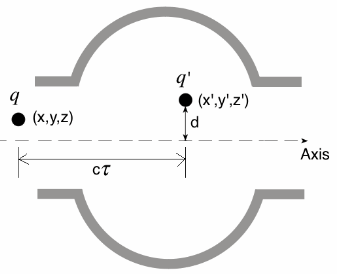
\includegraphics[width=0.60\linewidth]{figs/wakefield.png}
%\end{figure}
%\end{frame}

%------------------------------------------------

\begin{frame}
\frametitle{Beam Breakup Theory}
\begin{itemize}
\item Particles will undergo a change in momentum $\Delta p$ in the transverse direction from a potential induced by the wake $V(t)$
\end{itemize}
\begin{equation}
\Delta p = \frac{e}{c} V(t)
\end{equation}
\begin{itemize}
\item and a corresponding displacement at the same location the next pass
\end{itemize}
\begin{equation}
x = M_{12} \frac{\Delta p}{p}
\end{equation}
\begin{itemize}
\item where $M_{12}$ is the transfer matrix element. Beam can lose stability if not properly damped
\end{itemize}
%\begin{figure}
%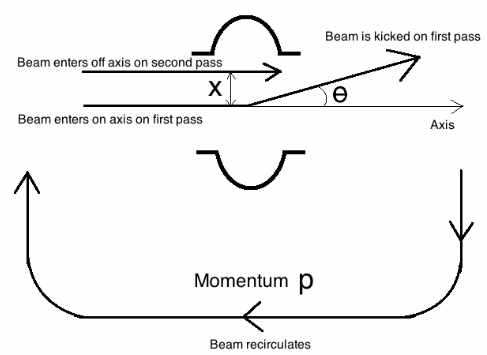
\includegraphics[width=0.60\linewidth]{figs/recirculation.png}
%\end{figure}
\end{frame}

%------------------------------------------------

\begin{frame}
\frametitle{Damping HOMs}
\begin{itemize}
\item HOMs must be damped for beam stability!
\item CEBAF uses waveguide dampers to damp the HOMs
\end{itemize}
\begin{figure}
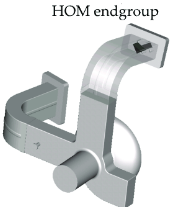
\includegraphics[width=0.30\linewidth]{figs/HOM.png}
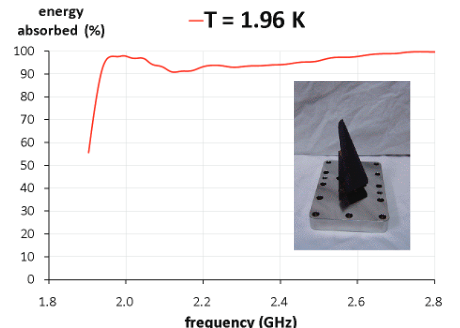
\includegraphics[width=0.50\linewidth]{figs/energy_absorbed.png}
\end{figure}
\end{frame}

%------------------------------------------------

\begin{frame}
\frametitle{Threshold Current}
\begin{itemize}
\item There is a \textbf{maximum current in the accelerator before beam becomes unstable}
\item Using how multiple particles produce and react to wake, the 1st order current threshold $I_{th}$ is given by 
\end{itemize}
\begin{equation}
I_{th}=-\frac{2pc/e}{(R/Q)_{\lambda} Q_{\lambda} k_{\lambda} M_{12} \sin{(\omega_{\lambda} T_r)} e^{\frac{\omega{\lambda}T_r}{2 Q_{\lambda}}}}
\end{equation}
\begin{itemize}
\item where $T_r$ is the revolution period
\item This diverges (and becomes negative) at certain frequecies, need the second order solution
\end{itemize}
\end{frame}

%------------------------------------------------

\begin{frame}
\frametitle{Threshold Current}
\begin{itemize}
\item The $I_{th}$ as a function of frequency for first order solution (blue), second order solution (green), and simulation (black)
\item The mimimum $I_{th}$ (red dot) is about 10 mA which is orders of maginitude above the design of 200$\mu$A
\end{itemize}
\begin{figure}
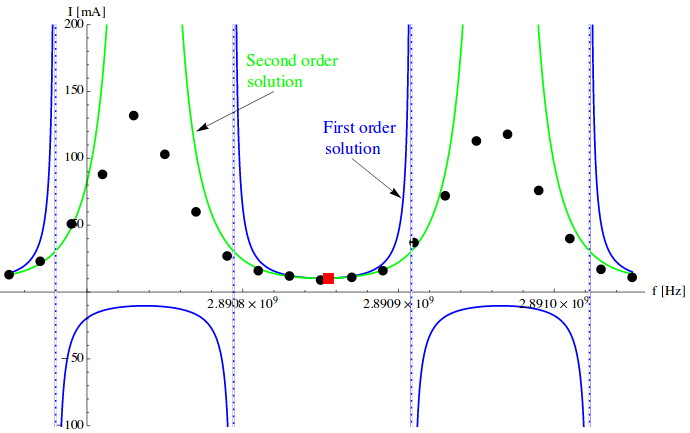
\includegraphics[width=0.80\linewidth]{figs/threshold.png}
\end{figure}
\end{frame}

%------------------------------------------------

%\begin{frame}
%\frametitle{HPS Beamline}
%\begin{itemize}
%\item Double-sided septum separates beam pulses into different experimental halls
%\end{itemize}
%\begin{figure}
%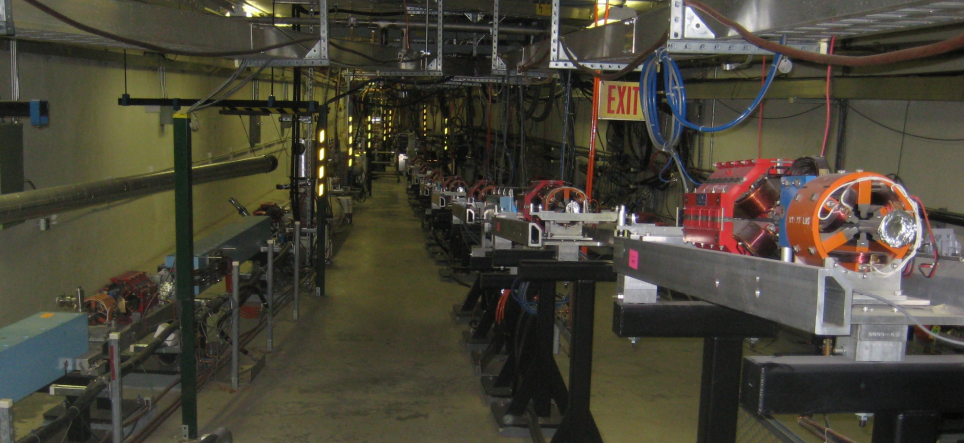
\includegraphics[width=0.60\linewidth]{figs/HallA_beamline.png}
%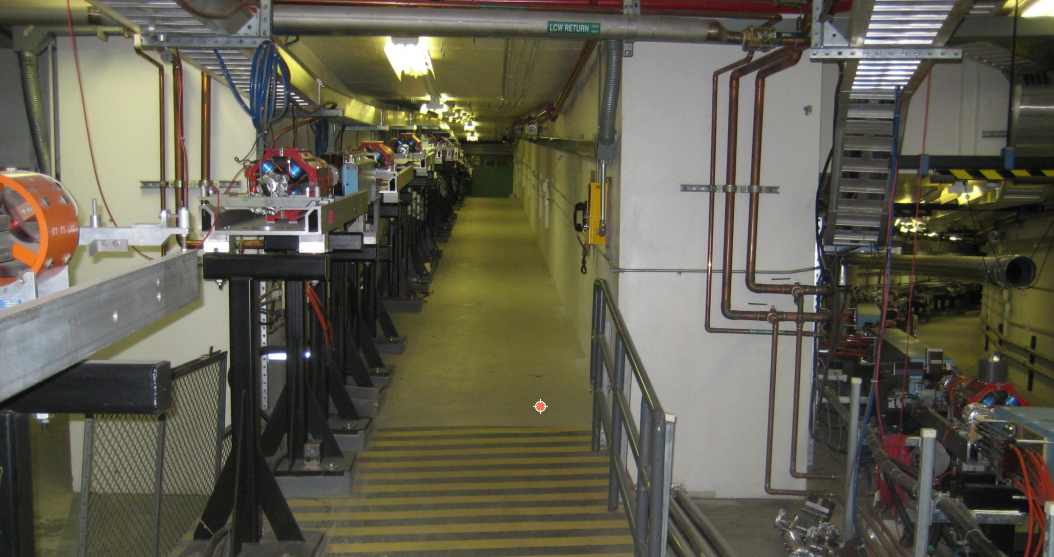
\includegraphics[width=0.52\linewidth]{figs/HallB_beamline.png}
%\end{figure}

%\end{frame}

%------------------------------------------------

%\begin{frame}
%\frametitle{HPS Beamline}
%\begin{itemize}
%\item HPS runs parasitically in Hall B (right) from Hall A (left)
%\end{itemize}
%\begin{figure}
%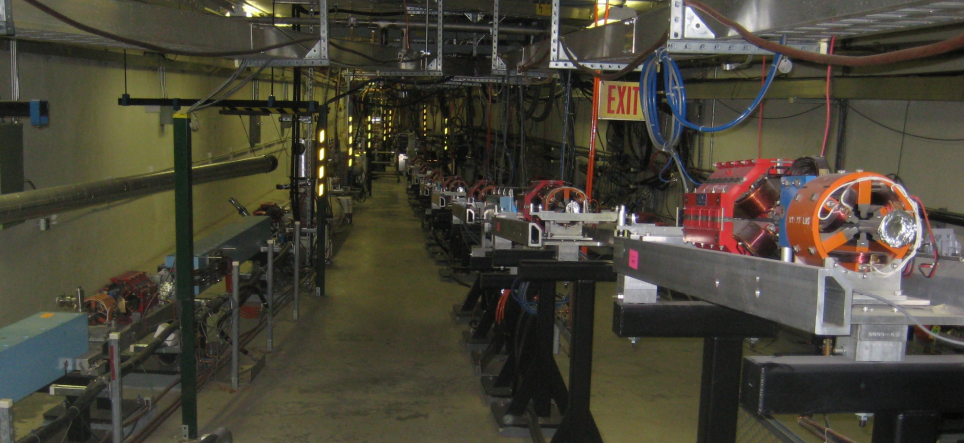
\includegraphics[width=0.60\linewidth]{figs/HallA_beamline.png}
%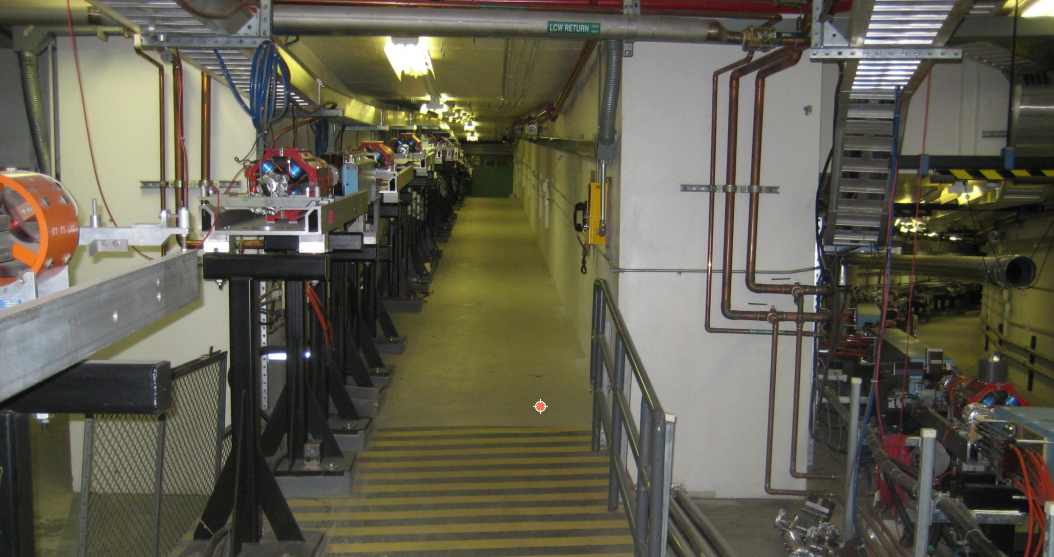
\includegraphics[width=0.52\linewidth]{figs/HallB_beamline.png}
%\end{figure}

%\end{frame}

%------------------------------------------------

\begin{frame}
\frametitle{Hall B Beamline}
\begin{itemize}
\item Hall B beamline consists of harp and wire scanners, tagger magnet, collimators, Clas12 detector, HPS dipole/chicane magnet, Faraday Cup, and beam dump
\item Tagger magnet dumps beam into ground while beam is tuned
\end{itemize}
\begin{figure}
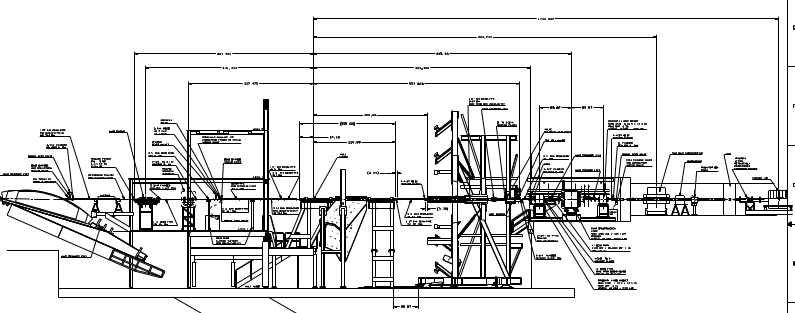
\includegraphics[width=1.00\linewidth]{figs/tagger.png}
\end{figure}

\end{frame}

%------------------------------------------------

\begin{frame}
\frametitle{HPS Beamline}
\begin{itemize}
\item Harp/wire scans measure beam profile before sending it to HPS
\item Chicane magnet steers beam to beam dump/Faraday Cup
\item Faraday cup measures total integrated current
\end{itemize}
\begin{figure}
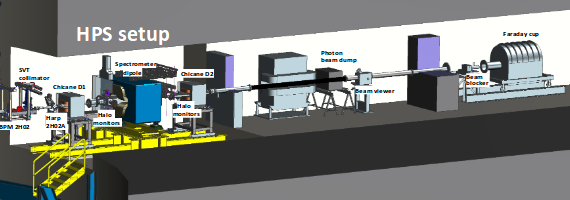
\includegraphics[width=1.00\linewidth]{figs/HPS_beamline.png}
\end{figure}

\end{frame}

%------------------------------------------------

\begin{frame}
\frametitle{Harp Scans 2016 Data}
\begin{itemize}
\item 2C21 harp scan before tagger (left) and 2H02 harp scan 2.2 m before target (right)
\end{itemize}
%\begin{figure}
%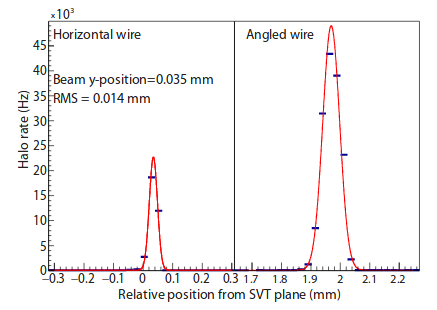
\includegraphics[width=0.40\linewidth]{figs/wire_scan.png}
%\end{figure}
\begin{figure}
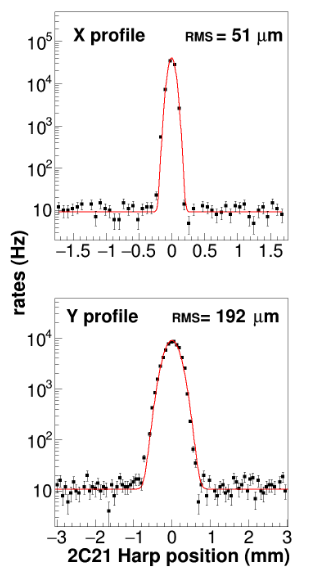
\includegraphics[width=0.30\linewidth]{figs/2C21_Harp.png}
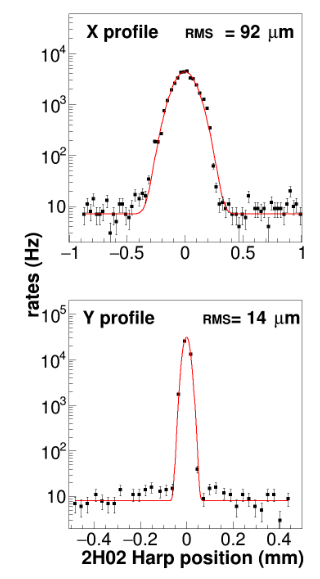
\includegraphics[width=0.30\linewidth]{figs/2H02_harp.png}
\end{figure}

\end{frame}

%------------------------------------------------

\begin{frame}
\frametitle{Beam Halo 2016 Data}
\begin{itemize}
\item Measurement of beam halo in 2016 data. Red is gaussian core of beam, green is occupancies (rates) in 1st tracking layer with target, blue is occupancies in 1st layer without target, and fitted blue is fitted beam halo
\end{itemize}
\begin{figure}
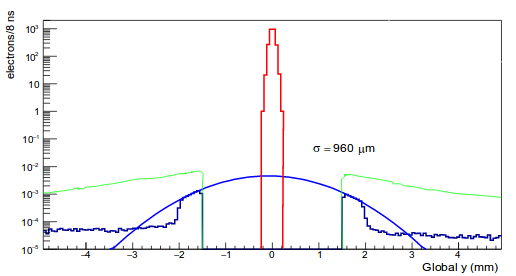
\includegraphics[width=0.60\linewidth]{figs/beam_halo.png}
\end{figure}

\end{frame}

%------------------------------------------------

\begin{frame}
\frametitle{Conclusion}
\begin{itemize}
\item CEBAF provides, and has been providing, sufficient electron beams for experiments on the interface between nuclear and particle physics
\item Large scale srf and recirculation technology put CEBAF on the forefront of accelerator physics
\item CEBAF recently underwent a 12 GeV upgrade from the 6 GeV machine
\item HPS has had two successful runs at different energies at CEBAF (1.05 GeV and 2.3 GeV), and \textbf{HPS looks forward to more beam time in 2018 and beyond}
\end{itemize}

\end{frame}

%------------------------------------------------

\begin{frame}
\frametitle{References}
\begin{itemize}
\item http://uspas.fnal.gov/materials/08UMD/Recirculating&ERLs.pdf
\item https://arxiv.org/pdf/1612.07821.pdf
\item http://iopscience.iop.org/article/10.1088/1742-6596/299/1/012015/pdf
\item https://www.jlab.org/div_dept/physics_division/talks/Background/Accelerator/CEBAF_Ann_Rev_2001.pdf
\item http://uspas.fnal.gov/materials/12UTA/Cathode_2.pdf
\item http://digitalcommons.uconn.edu/cgi/viewcontent.cgi?article=6258&context=dissertations
\item https://www.jlab.org/indico/event/98/contribution/3/material/slides/0.pdf
\end{itemize}

\end{frame}

%------------------------------------------------

\end{document} 
